\clearpage
\setcounter{page}{1}
\maketitlesupplementary


\section{Smoothness Proof Sketch}
A Delaunay triangulation can be formed by taking a triangulation and then flipping the edges of triangles that are not Delaunay (e.g.\ the edges that have a circumsphere containing a vertex)~\cite{hurtado1996flipping}. In 3D, these edge-flips are called Pachner moves~\cite{pachner1991pl}.
As discussed in Sec.~\ref{sec:query},
% during a Delaunay triangulation arbitrary edge flips may occur
during optimization we make take a valid Delaunay triangulation and then move the vertices by some small amount $\epsilon$
such that a vertex may enter the circumsphere of a neighboring tetrahedron, thereby triggering a topological flip.
% by some $\epsilon$, a flip may take place when a circumsphere from the previous triangulation now contains a vertex.
This implies that the vertex was already nearby the circumsphere boundary prior to the move. 
% For this to have happened, the offending vertex must have been close to the offending circumsphere. 
% If we form a triangle using the offending vertex and any of the vertices from the offending circumsphere, then it must form a circumsphere similar to the offending circumsphere. Therefore, the flip must have been caused by points from a similar circumsphere.
Consequently, these flips must involve sets of points that are nearly cospherical, as the geometric configurations before and after the flip share an almost identical circumsphere.

\section{Sorting Proof Sketch}
% To show by induction how we can sort a Delaunay triangulation using powers of circumspheres, we sort two arbitrary adjacent triangles which are not contained within each other's circumspheres.
% If two triangles satisfy the empty circumsphere property, we can always depict them using two circles where one edge lines along the intersection between the two circles, and the rest of each triangle lies on the other side of their respective circle. The intuition here is that the line of equal power, or the radical axis, lies along this shared edge. This also happens to be the line along which the sort order changes. It is then trivial to show that the power of the further primitive increases relative to the closer one, thereby yielding the correct sort order for the two primitives. This proof generalizes to 3D.
To demonstrate how a Delaunay triangulation can be visibility-sorted relative to a specific viewpoint using the power of circumcircles, consider two adjacent triangles. Geometrically, the edge shared by these two triangles lies along the radical axis (the line of intersection) of their respective circumcircles.
This axis is the line of equal power; it divides the plane into two regions. On one side, the viewpoint has a lower power distance to the first circumcircle, but on the other side it has a lower power distance to the second. Since the relative depth order of the two triangles flips only when the viewpoint crosses this axis, the power distance serves as a consistent sorting criterion. This implies that sorting the primitives by the power of the viewpoint relative to their circumcircles yields the correct visibility order. This property naturally generalizes to 3D, where the shared face of two tetrahedra lies on the radical plane. See Figure~\ref{fig:radical_axis} for a visualization.

\begin{figure}[h]
    \centering
    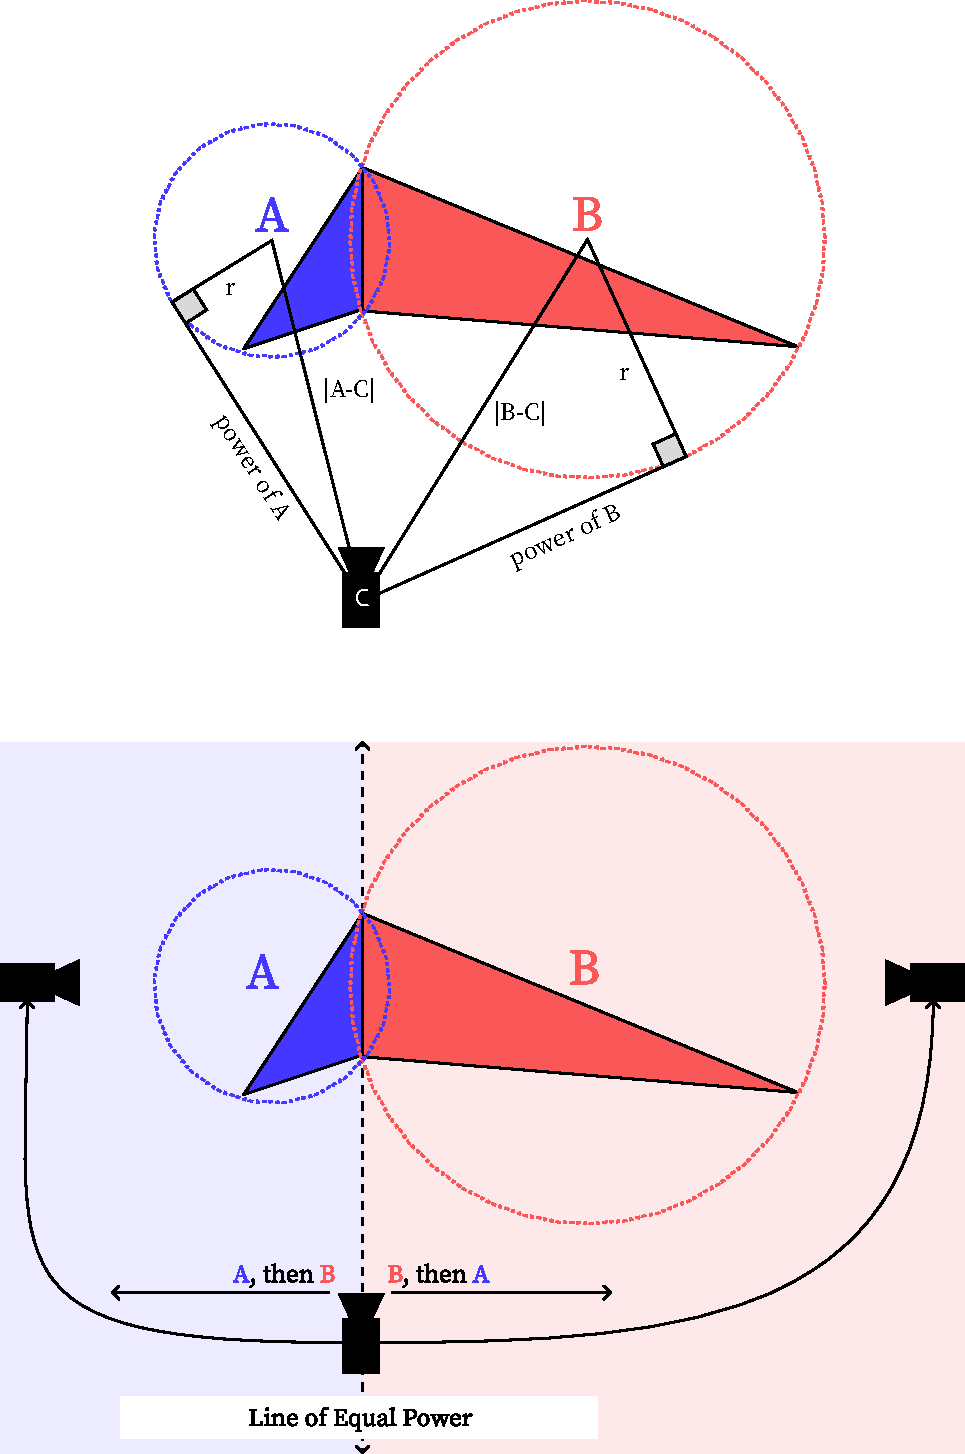
\includegraphics[width=\linewidth]{figures/sorting_diagram.pdf}
    \caption{To sort two adjacent triangles relative to a viewpoint, we need only look at their circumcircles. The radical axis (the line along which the power of a spheres is equal) goes through the two intersection points between the circles, and divides the circumscribed triangles.
    Consider the centers of two circumcircles $A$ and $B$ and a viewpoint $C$ located along the radical axis.
    Since $|A-C|$ increases as the camera moves right and $|B-C|$ decreases, the power of B is less than the power of A to the right, and the reverse is true to the left. This extends to non-intersecting circles, and can be used for non adjacent triangles. Combining this observation with the the Delaunay empty sphere property allows us to sort all triangles.
    }
    \label{fig:radical_axis}
\end{figure}

\section{Details}

% Combined with the viewing direction, this means we have our function $f_\theta$ has domain: circumcenter $\in R^3$, radius $\in R_{>0}$, viewing direction $\in R^3$. 
% Putting it all together, during optimization, the scene is represented by the following optimizable parameters: a set of 3D points $\mathcal{X}$ and a neural network weights $\theta$.
% The 3D Delaunay triangulation of these points yields a set of tetrahedra $\{T_k\}_{k=1}^N$.
% These tetrahedra can then be associated with a constant density and linearly varying color by querying $f_\theta$ at the circumcenter $\circumcenter_k$ and corresponding circumradius $\circumradius_k$, ith viewing direction $d_k = \frac{\centroid_k - o}{\|\centroid_k - o\|}$, where $\centroid_k$ is the centroid of tetrahedron $k$:
% \[
% \{\sigma_k, \colorc_k, \cgradient_k\} = f_\theta\left( \stopnabla{}  \circumcenter_k, \stopnabla{} \circumradius_k, \stopnabla{} d_k\right)
% \]
% where \(\sigma_k\in\mathbb R_{\ge0}\) is the constant density, \(\colorc_k\in\mathbb R^3\) is the base color centered at the circumsphere center, \(\cgradient\in\mathbb R^3\) is the monochromatic color gradient, and $\stopnabla{}$ is the stop gradient symbol.

% We stop the gradient across these inputs into $f$ to avoid determining the position of the vertices according to the linear interpolation gradients, which are noisy from the hash function.

Even though we are using GPU acceleration, recomputing a Delaunay triangular from scratch is still somewhat slow.
As such, we only update vertex locations and their corresponding Delaunay topology every 10 iterations.
On a scene with 1.2 million tetrahedra, our timings during training are approximately 19 milliseconds for rendering, 13 milliseconds to query the instant-NGP, 143 milliseconds for the backwards pass, and 92 milliseconds to compute the Delaunay triangulation.

Because densification changes the circumcenters of the primitives and therefore their colors, we temporarily increase the learning rate of some of the model to allow it to rapidly  accommodate for this change.
After densification at iteration $I$, we increase the learning rate of the instant NGP weights and the vertex coordinates
% $\theta$ and $\mathcal{X}$
by adding a ``spike'' function with duration $L$ on top of the decay function $l(i)$:
\begin{align}
    \mathbbm{1}\{i-I>0\}\left(l(0) - l(I)\right)\exp\left(-\frac{6(i-I)}{L}\right)
\end{align}
This increases the decaying learning rate back up to its maximum (initial) value, before decaying it back down in $L$ iterations.


\subsection{Algorithm Details}\label{sec:rasterization-details}
The naive version of our shader would, for each of the 4 vertices of each tetrahedra, load all of the tetrahedra information and attached it each of the vertices.
Then, when the fragment shader for any given triangle is called, the information from the closest vertex would be obtained, and the full Cyrus-Beck algorithm~\cite{cyrus1978} would be run on the rest of the tetrahedra to compute the back intersection, which then allows us to compute the integral along the intersection with the primitive.

In our optimized implementation, we leverage the capabilities of a mesh shader to allow the four vertices of each tetrahedra to share information between themselves. This reduces the number of loads by a factor of four. We also optimize the Cyrus-Beck algorithm: in the vertex shader we precompute the intersection distance with each of the vertices, and then perform interpolation between these distances to find the intersection distance with each plane. This interpolation must be perspective-correct barycentric interpolation to ensure that the interpolation results are correct. A similar technique can be applied to the color gradient to further simplify the fragment shader.
This reduces runtime cost to only 12 FLOPs. See Algorithm~\ref{alg:shader}.

\begin{algorithm}[htbp]
    \caption{Shader code to perform accelerated intersections using wave intrinsics within a mesh shader.}
    \label{alg:shader}

    % --- Block 1: Mesh Shader ---
    \begin{lstlisting}[title={Mesh shader intersection pre-calculation}]
uint bli = (WaveGetLaneIndex() / 4) * 4;
#define WRTV(x, id) WaveReadLaneAt(x, bli + id)

static const uint4 kTetTriangles[4] = {
    uint4(0, 2, 1, 3),
    uint4(1, 2, 3, 0),
    uint4(0, 3, 2, 1),
    uint4(3, 0, 1, 2),
};

tri = kTetTriangles[tetVertexId];

// outward facing normal
n = cross(
    WRTRV(vertex, tri[2]) -
    WRTRV(vertex, tri[0]),
    WRTRV(vertex, tri[1]) -
    WRTRV(vertex, tri[0]));

v = WRTRV(vertex, tri[0])
num = dot(n, v - rayOrigin);

o.planeN = float4(
    WRTRV(num, 0),
    WRTRV(num, 1),
    WRTRV(num, 2),
    WRTRV(num, 3) );
o.planeD = float4(
    dot(WRTRV(n, 0), o.rayDir),
    dot(WRTRV(n, 1), o.rayDir),
    dot(WRTRV(n, 2), o.rayDir),
    dot(WRTRV(n, 3), o.rayDir) );
return o;
    \end{lstlisting}

    % --- Block 2: Fragment Shader ---
    \begin{lstlisting}[title={Fragment shader intersection routine}]
d = length(rayDir);
o.planeD /= d;

all_t = o.planeN / o.planeD;

t_enter = max(o.planeD > 0.0f ? all_t : -FLT_MAX);
t_exit  = min(o.planeD < 0.0f ? all_t : FLT_MAX);
    \end{lstlisting}

\end{algorithm}

% \begin{algorithm}[htbp]
%     \caption{Shader code to perform accelerated intersections using wave intrinsics within a mesh shader.
%     }
%     \label{alg:shader}
% \begin{minted}
% [frame=lines,
%  framerule=1pt,
%  % rulecolor=\color{black!20},
%  label={Mesh shader intersection pre-calculation},
%  fontsize=\footnotesize]
% {hlsl}
% uint bli = (WaveGetLaneIndex() / 4) * 4;
% #define WRTV(x, id) WaveReadLaneAt(x, bli + id)

% static const uint4 kTetTriangles[4] = {
%     uint4(0, 2, 1, 3),
%     uint4(1, 2, 3, 0),
%     uint4(0, 3, 2, 1),
%     uint4(3, 0, 1, 2),
% };

% tri = kTetTriangles[tetVertexId];

% // outward facing normal
% n = cross(
%     WRTRV(vertex, tri[2]) -
%     WRTRV(vertex, tri[0]),
%     WRTRV(vertex, tri[1]) -
%     WRTRV(vertex, tri[0]));

% v = WRTRV(vertex, tri[0])
% num = dot(n, v - rayOrigin);

% o.planeN = float4(
%     WRTRV(num, 0),
%     WRTRV(num, 1),
%     WRTRV(num, 2),
%     WRTRV(num, 3) );
% o.planeD = float4(
%     dot(WRTRV(n, 0), o.rayDir),
%     dot(WRTRV(n, 1), o.rayDir),
%     dot(WRTRV(n, 2), o.rayDir),
%     dot(WRTRV(n, 3), o.rayDir) );
% return o;
% \end{minted}

% \begin{minted}
% [frame=lines,
%  framerule=1pt,
%  % rulecolor=\color{black!20},
%  label={Fragment shader intersection routine},
%  fontsize=\footnotesize]
% {hlsl}
% d = length(rayDir);
% o.planeD /= d;

% all_t = o.planeN / o.planeD;

% t_enter = max(o.planeD > 0.0f ? all_t : -FLT_MAX);
% t_exit  = min(o.planeD < 0.0f ? all_t : FLT_MAX);
% \end{minted}
% % \end{figure}
% \end{algorithm}


\section{Results}

See Figure~\ref{fig:comparison_supp} for additional results.

\newcommand{\graphimone}[1]{
\begin{tikzpicture}[zoomboxarray, zoomboxarray rows=1, zoomboxes below, zoomboxarray inner gap=0.0cm]
    \node [image node] { \includegraphics[width=3.5cm,valign=b]{#1} };
    \zoombox[magnification=3]{0.25,0.18}
\end{tikzpicture}
}

\newcommand{\graphimtwo}[1]{
\begin{tikzpicture}[zoomboxarray, zoomboxarray rows=1, zoomboxes below, zoomboxarray inner gap=0.0cm]
    \node [image node] { \includegraphics[width=3.5cm,valign=b]{#1} };
    \zoombox[magnification=5]{0.35,0.87}
\end{tikzpicture}
}

\newcommand{\graphimthree}[1]{
\begin{tikzpicture}[zoomboxarray, zoomboxarray rows=1, zoomboxes below, zoomboxarray inner gap=0.0cm]
    \node [image node] { \includegraphics[width=3.5cm,valign=b]{#1} };
    \zoombox[magnification=4]{0.80,0.55}
\end{tikzpicture}
}

\newcommand{\graphimfour}[1]{
\begin{tikzpicture}[zoomboxarray, zoomboxarray rows=1, zoomboxes below, zoomboxarray inner gap=0.0cm]
    \node [image node] { \includegraphics[width=3.5cm,valign=b]{#1} };
    \zoombox[magnification=3]{0.45,0.36}
\end{tikzpicture}
}

\begin{figure*}[ht]
\centering
\bgroup
% \def\arraystretch{2}
\begin{tabular}{@{}c@{}c@{}c@{}c@{}c@{}}
\graphimone{comparison_table_jpg/3dgs_00016.jpg} &
\graphimone{comparison_table_jpg/ever_00016.jpg} &
\graphimone{comparison_table_jpg/rf_00016.jpg} &
\graphimone{comparison_table_jpg/rm_00016.jpg} &
\graphimone{comparison_table_jpg/gt_00016.jpg} \\
\graphimtwo{comparison_table_jpg/3dgs_00001.jpg} &
\graphimtwo{comparison_table_jpg/ever_00001.jpg} &
\graphimtwo{comparison_table_jpg/rf_00001.jpg} &
\graphimtwo{comparison_table_jpg/rm_00001.jpg} &
\graphimtwo{comparison_table_jpg/gt_00001.jpg} \\
\graphimthree{comparison_table_jpg/3dgs_00028.jpg} &
\graphimthree{comparison_table_jpg/ever_00028.jpg} &
\graphimthree{comparison_table_jpg/rf_00028.jpg} &
\graphimthree{comparison_table_jpg/rm_00028.jpg} &
\graphimthree{comparison_table_jpg/gt_00028.jpg} \\
\graphimfour{comparison_table_jpg/3dgs_00014.jpg} &
\graphimfour{comparison_table_jpg/ever_00014.jpg} &
\graphimfour{comparison_table_jpg/rf_00014.jpg} &
\graphimfour{comparison_table_jpg/rm_00014.jpg} &
\graphimfour{comparison_table_jpg/gt_00014.jpg} \\
3DGS & EVER & RadiantFoam & Ours & GT
\end{tabular}
\egroup
\caption{Visual comparison of our method alongside baseline algorithms on various scenes from the datasets we use.}
\label{fig:comparison_supp}
\end{figure*}
